\section{El problema del viajante de comercio}

El problema del viajante de comercio consiste en hallar el recorrido con distancia
mínima en un conjunto de ciudades que pase por todas las ciudades y regrese al punto
inicial. \\

La implementación de los algoritmos es de la forma:
\begin{description}
 \item[Entrada:] Ficheros con ciudades indicadas como puntos en el plano según sus
 coordenadas.
 \item[Salida:] \texttt{vector<int>} con el orden en el que se recorren las ciudades.
\end{description}

En la salida nos ahorraremos repetir el primer nodo al final del recorrido.

Para todos los algoritmos utilizaremos una estructura de datos que nos permita manejar
el problema: la clase \texttt{Grafo} (en el fichero \texttt{grafo.h}). Un grafo consta
de:

\begin{itemize}
  \item Una \textbf{cantidad de nodos}, almacenada en el atributo \texttt{nodos}.
  \item Una \textbf{matriz de pesos}, almacenada en el vector \texttt{lados}.
\end{itemize}

La interfaz nos permite acceder y modificar estos datos con mayor facilidad.
Mediante los métodos \texttt{setPeso} y \texttt{peso} accederemos al peso de un
lado del grafo, y el método \texttt{pesosDesdeCoordenadas} nos permite inicializar el
grafo utilizando el formato de datos en el que aparece el problema: calculando
la distancia entre cualesquiera dos ciudades y añadir esta como peso de ese lado:

\lstinputlisting[firstline=47, lastline=51]{cpps/grafo.h}

Adicionalmente, la función \texttt{longitud} calcula la longitud de un camino dado,
teniendo en cuenta la distancia del último nodo al primero:

\lstinputlisting[firstline=54, lastline=59]{cpps/grafo.h}

Siendo \texttt{peso\_t} el tipo de dato con el que se manejen las distancias entre
nodos. Según el enunciado del problema (que pide que se redondee la distancia
euclídea al entero más próximo), será de tipo \texttt{int}.

\subsection{Ramificación y acotación}

El primer tipo de algoritmos a implementar son los algoritmos de ramificación y acotación
(\textit{branch and bound}). Estos algoritmos exploran un árbol de caminos parciales (en el que los hijos de un nodo añaden una ciudad no visitada) pero expandiendo solo aquellos nodos para los que existe la posibilidad de que haya una solución mejor que la mejor
encontrada hasta el momento. \\

En primer lugar veremos el algoritmo de ramificación y acotación para una cota general y por último veremos la implementación de las cotas que hemos utilizado.

\subsubsection{Algoritmo general}

Presentamos en esta sección un algoritmo general que implementa el \textit{branch and bound} dada una función de acotación. Utilizaremos este mismo algoritmo variando únicamente la función de cota para las dos implementaciones. En casos particulares en los que existe una forma eficiente de obtener la cota de una solución parcial a partir de la de su padre (la solución parcial que tiene todas las ciudades menos la última), podrían hacerse pequeñas modificaciones de este algoritmo para optimizar el cálculo de la misma. \\

El algoritmo toma un \texttt{Grafo} y una función \texttt{cota}. Esta última calcula a partir de un camino (y el grafo) un entero que será menor o igual que la mejor solución posible que pueda obtenerse añadiendo nuevas ciudades a la solución parcial. La distancia del valor obtenido a la longitud de la mejor solución posible y el tiempo requerido para obtenerlo determinarán el tiempo de ejecución del algoritmo.  \\

En primer lugar iniciamos la cola con prioridad introduciendo el camino parcial
inicial (\texttt{[0]}). Para optimizar el cálculo guardamos también en la cola el valor de la cota para cada nodo que introducimos. Inicializamos la mejor solución encontrada con un algoritmo greedy (en este caso, vecino más cercano).

\begin{lstlisting}
priority_queue<pair<vector<int>,int>,vector<pair<vector<int>,int> >,Compare> cola;
vector<int> inicial = {0}, mejor_camino = tsp_greedy(g);
int mejor_longitud = longitud(mejor_camino,g);
cola.push({inicial,cota(inicial,g)});
\end{lstlisting}

A partir de aquí, mientras la cola no esté vacía cogemos el nodo en el frente (aquel con menor cota) y distinguimos dos casos: \\

Si \textbf{basta añadir 2 ciudades para hallar un camino}, creamos todos los caminos posibles y comprobamos, para cada uno de ellos, si es mejor que la mejor solución encontrada hasta el momento, y en tal caso actualizamos la mejor solución. Esto permite no añadir más nodos a la cola de prioridad y genera una ligera mejora en los tiempos de ejecución.

\begin{lstlisting}
for(int i = 0; i < g.numNodos(); i++){
  if(find(camino_actual.begin(), camino_actual.end(), i) == camino_actual.end()){
    vector<int> pos_sol = camino_actual;
    pos_sol.push_back(i);

    // Añade el otro nodo
    bool encontrado = false;
    for(int j = 0; !encontrado && j < g.numNodos(); j++){
      if(find(pos_sol.begin(), pos_sol.end(), j) == pos_sol.end()){
        pos_sol.push_back(j);
        encontrado = true;
      }
    }

    int long_sol = longitud(pos_sol, g);

    // Actualiza la mejor solución
    if(long_sol < mejor_longitud){
      mejor_longitud = long_sol;
      mejor_camino = pos_sol;
    }
  }
}
\end{lstlisting}

En el caso de que \textbf{no baste añadir 2 ciudades a la solución parcial} que estamos considerando, para cada ciudad no visitada consideramos el camino que resulta de añadir esta ciudad al final de la solución parcial. Si la nueva solución tiene una cota menor que la de la mejor solución la insertamos ordenadamente en la cola:

\begin{lstlisting}
for(int i = 0; i < g.numNodos(); i++){
  if(find(camino_actual.begin(), camino_actual.end(), i) == camino_actual.end()){
    vector<int> nuevo_camino = camino_actual;
    nuevo_camino.push_back(i);

    int nueva_cota = cota(nuevo_camino,g);
    if(nueva_cota < mejor_longitud)
      cola.push({nuevo_camino,nueva_cota});
  }
}
\end{lstlisting}

Repetimos este proceso y devolvemos el mejor camino encontrado. El algoritmo completo queda:

\begin{lstlisting}
vector<int> tsp_cota(const Grafo<peso_t>& g, int (*cota)(vector<int>&, const Grafo<int>&)) {
  priority_queue<pair<vector<int>,int>,vector<pair<vector<int>,int> >,Compare> cola;
  vector<int> inicial = {0}, mejor_camino = tsp_greedy(g);
  int mejor_longitud = longitud(mejor_camino,g);
  cola.push({inicial,cota(inicial,g)});

  // Mientras haya caminos posiblemente mejores que el mejor encontrado
  while((!cola.empty()) && (cola.top().second < mejor_longitud)){

    vector<int> camino_actual = cola.top().first;
    cola.pop();
    // No podemos formar directamente una solución
    if(camino_actual.size() < g.numNodos()- 2){
      for(int i = 0; i < g.numNodos(); i++){
        if(find(camino_actual.begin(), camino_actual.end(), i) == camino_actual.end()){
          vector<int> nuevo_camino = camino_actual;
          nuevo_camino.push_back(i);

          int nueva_cota = cota(nuevo_camino,g);
          if(nueva_cota < mejor_longitud)
            cola.push({nuevo_camino,nueva_cota});
        }
      }
    }
    else{// Podemos formar una solución
      for(int i = 0; i < g.numNodos(); i++){
        if(find(camino_actual.begin(), camino_actual.end(), i) == camino_actual.end()){
          vector<int> pos_sol = camino_actual;
          pos_sol.push_back(i);

          // Añade el otro nodo
          bool encontrado = false;
          for(int j = 0; !encontrado && j < g.numNodos(); j++){
            if(find(pos_sol.begin(), pos_sol.end(), j) == pos_sol.end()){
              pos_sol.push_back(j);
              encontrado = true;
            }
          }

          int long_sol = longitud(pos_sol, g);

          // Actualiza la mejor solución
          if(long_sol < mejor_longitud){
            mejor_longitud = long_sol;
            mejor_camino = pos_sol;
          }
        }
      }
    }
  }
  return mejor_camino;
}
\end{lstlisting}

\subsubsection{Cotas}

Para implementar la función de acotación pedida en el enunciado utilizamos una función auxiliar \texttt{RelacionadosCon} que nos indica, dada una ciudad, cuál es el conjunto de ciudades que debemos considerar para calcular la cota:

\begin{lstlisting}
vector<int> RelacionadosCon(int k, int max, vector<int> camino){
  vector<int> relacionados;
  for(int i = 0; i < max; i++)
    if(find(camino.begin(), camino.end(), i) == camino.end() && i != k)
      relacionados.push_back(i);
  if(k != camino.back() || k == max-1)
    relacionados.push_back(1);
  return relacionados;
}
\end{lstlisting}

De esta forma calcular la primera cota se reduce a calcular la longitud del recorrido inicial y sumar la menor distancia de cada ciudad no incluida en la solución parcial con sus relacionadas:

\begin{lstlisting}
int cota1(vector<int>& camino, const Grafo<int>& g){
  int recorrido = 0;
  for(int i = 0; i < camino.size()-1; i++)
    recorrido += g.peso(camino[i], camino[i+1]);

  for(int i = 0; i < g.numNodos(); i++){
    if((i == camino.back()) || (find(camino.begin(), camino.end(), i) == camino.end())){
      vector<int> v = RelacionadosCon(i,g.numNodos(),camino);
      int min = v[0];
      for(int j = 1; j < v.size(); j++){
        if(g.peso(i,v[j]) < g.peso(i,min))
          min = v[j];
      }
      recorrido += g.peso(i,min);
    }
  }
  return recorrido;
}
\end{lstlisting}

Se nos pedía además una función de cota original, y hemos optado por usar lo que sabíamos de árboles generadores minimales de los grafos. Así que la segunda cota toma el recorrido del camino parcial que se tiene hasta ese momento y le suma el recorrido del árbol generador minimal de los nodos que faltan por meter junto al último nodo del camino. Como el árbol generador minimal es la forma más corta de comunicar los nodos que faltan, no vamos a poder realizar un camino que pase por ellos que sea menor que eso, así que es una cota real del camino mínimo. \\

Para calcular la cota usamos el algoritmo de Kruskal, que toma en cuenta el peso de las aristas y las va cogiendo en orden, excluyendo aquellas que formen ciclos al ser incluidas. Se puede ver que el método no dista mucho de la primera cota, puesto que muchas de las aristas que coja el primero se cogerán en este, ya que las ordenan por la misma comparación. Hay que notar que la primera cota podía formar ciclos o incluso no llegar a formar un camino, mientras que esta segunda cota garantiza la conexión entre los nodos (y por un único camino). \\

Si bien ganamos en la acotación %% TODO: (Antonio) Comprobar que de verdad se gana, que no estoy seguro)
la eficiencia es algo peor que en el primer caso. Debido a que el algoritmo se vuelve inservible a partir de muy pocos nodos (cerca de 16), la eficiencia de la cota en función de los nodos no debería afectar tanto al resultado. %% Aunque sí que afecta, JAJ
\\

La función de cota queda así:
\begin{lstlisting}
int cota2(vector<int>& camino, const Grafo<int>& g){
  int recorrido = 0;// Peso del recorrido ya hecho
  vector<vector<pair<int,int> > > aristas;
  vector<pair<int,int> > arista;
  int total_aristas = camino.size()-1;

  for(int i = 0; i < camino.size()-1; i++){
    recorrido += g.peso(camino[i], camino[i+1]);
    arista.push_back(pair<int,int>(camino[i],camino[i+1]));
   }
  aristas.push_back(arista);
  arista.clear();

  while(total_aristas < g.numNodos()-1){
    pair<int,int> par_nuevo = MenorAristaSiguiente(aristas, g);
    arista.push_back(par_nuevo);
    aristas.push_back(arista);
    recorrido += g.peso(par_nuevo.first, par_nuevo.second);
    RecomponerAristas(aristas);
    arista.clear();
    total_aristas++;
  }
  int minimo = INFINITO;
  for(int i = 1; i < g.numNodos(); i++)
    if(g.peso(0,i) < minimo && (find(camino.begin(), camino.end(), i) == camino.end()))
      minimo = g.peso(0,i);
  return recorrido + minimo;
}
\end{lstlisting}

\subsection{Vuelta atrás}

Con un camino y su longitud inicial se desarrolla el algoritmo de la vuelta atrás de la siguiente manera: desde un nodo inicial, vamos añadiendo nodo a nodo creando distintos caminos tomando todas las posibilidades mediante llamadas recursivas. Si, tras añadir un nodo, el camino mide más o lo mismo que nuestra mejor longitud hasta el momento se deja esa posibilidad y se miran otras posibilidades desde el nodo anterior al último. Es decir, se poda esa rama y se estudian las demás. Esto es, por definición, la vuelta atrás. \\

Si se llega a crear un camino completo que mida menos que nuestro camino más corto hasta el momento, este pasa a ser nuestro nuevo camino más corto. \\

Esta es la función que emplea la llamada recursiva, recibiendo una primera mejor longitud para tener un buen criterio de poda:

\begin{lstlisting}
void tsp_back_rec(vector<int>& solucion, vector<int> camino_actual, int& mejor_longitud, const Grafo<peso_t>& g){
  if(camino_actual.size() < g.numNodos()){
    for(int i = 0; i < g.numNodos(); i++){
      if(find(camino_actual.begin(), camino_actual.end(), i) == camino_actual.end()){
	      vector<int> nuevo_camino = camino_actual;
	      nuevo_camino.push_back(i);

        if(longitud(camino_actual,g) < mejor_longitud)
	        tsp_back_rec(solucion,nuevo_camino,mejor_longitud,g);
      }
    }
  }
  else{
    if(longitud(camino_actual,g) < mejor_longitud){
      mejor_longitud = longitud(camino_actual,g);
      solucion = camino_actual;
    }
  }
}
\end{lstlisting}

Y esta es la función que llama a la anterior, donde obtenemos la primera solución (mediante el algoritmo Greedy), y donde fijamos que el primer nodo será el de la posición \texttt{\{0\}}:

\begin{lstlisting}
vector<int> tsp_backtracking(const Grafo<peso_t>& g) {
	vector<int> primera_solucion = tsp_greedy(g);
	int mejor_longitud = longitud(primera_solucion,g);
	vector<int> inicial = {0};
	vector<int> solucion; // se modifica éste

	tsp_back_rec(solucion,inicial,mejor_longitud,g);

	return solucion;
}
\end{lstlisting}

Debemos notar que la longitud del camino más corto se pasa como referencia, pues se irá modificando mediante el algoritmo de vuelta atrás, y es importante tenerla presente todo el tiempo para podar correctamente.

\subsection{Comparativa de los algoritmos}

Seleccionados tres ejemplos con 5, 10 y 12 nodos, se va a comparar primero los caminos óptimos seleccionados por cada algoritmo, y después se hará una comparación de los datos (tiempo, etc.). Se ha de notar que las longitudes de los caminos óptimos es la misma, sea cual sea el algoritmo usado.

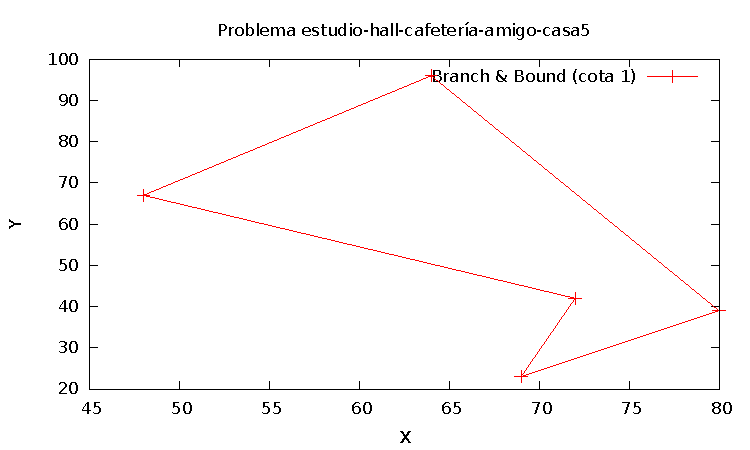
\includegraphics[width=15cm]{img/e-h-c-a-c5_tsp_1}

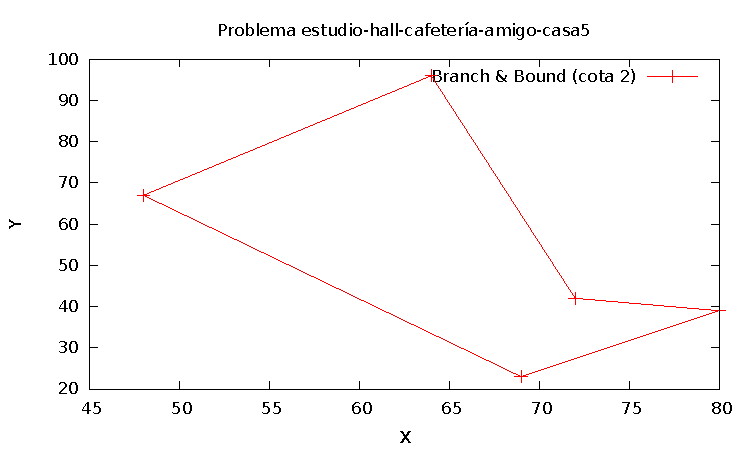
\includegraphics[width=15cm]{img/e-h-c-a-c5_tsp_2}

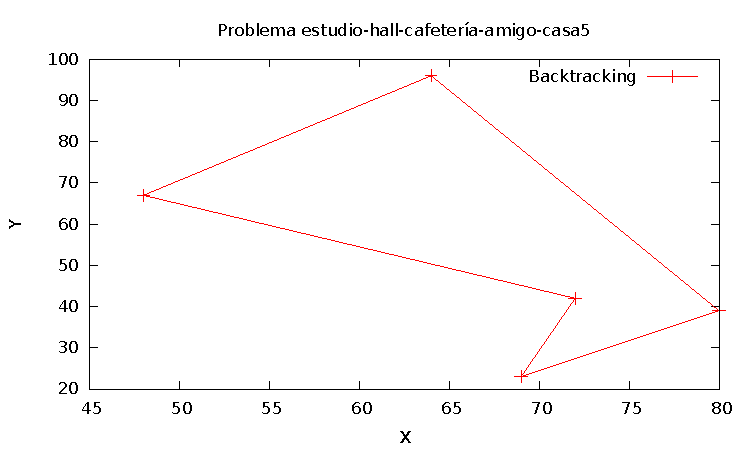
\includegraphics[width=15cm]{img/e-h-c-a-c5_tsp_3}

En este primer caso, el Branch and Bound con la primera cota y Backtracking coinciden, pero el del Branch and Bound con el Árbol generador no.

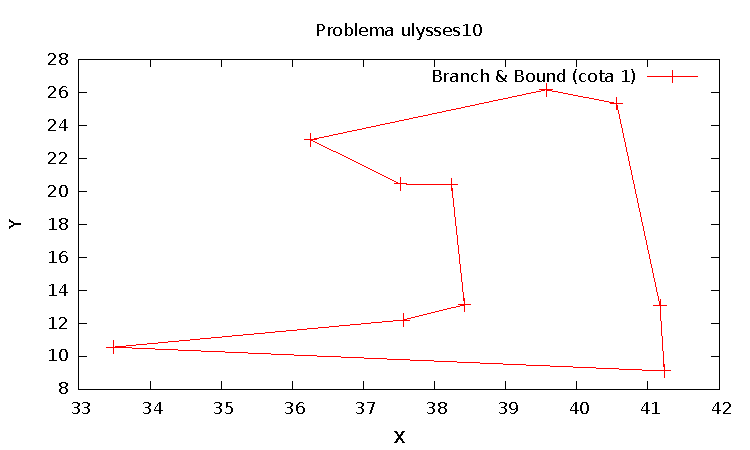
\includegraphics[width=15cm]{img/ulysses10_tsp_1}

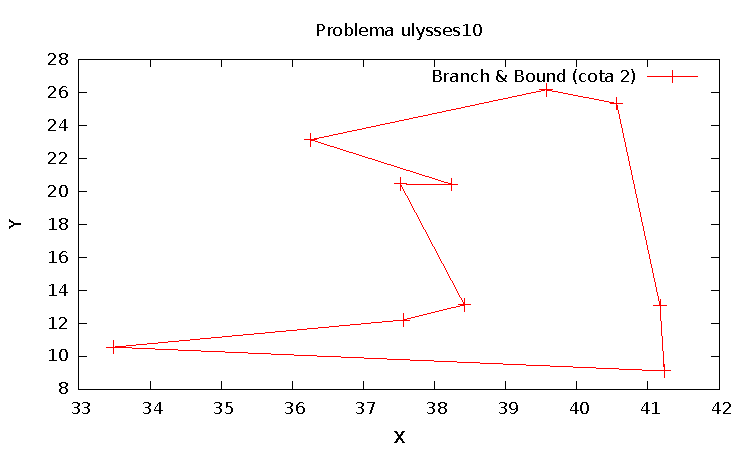
\includegraphics[width=15cm]{img/ulysses10_tsp_2}

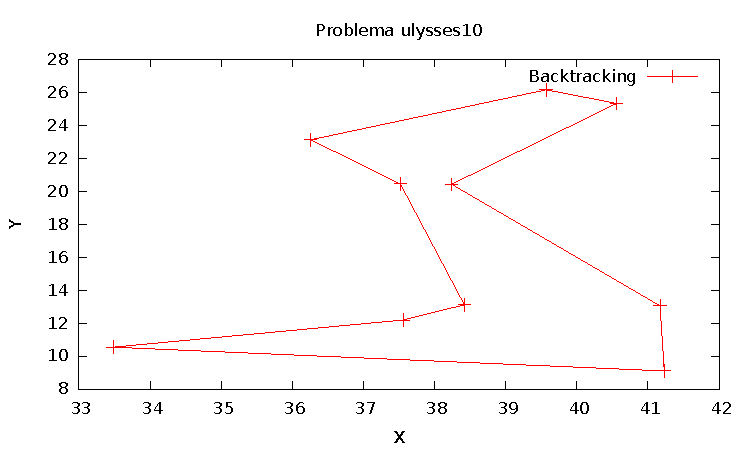
\includegraphics[width=15cm]{img/ulysses10_tsp_3}

En este segundo caso, cada algoritmo toma un camino distinto.

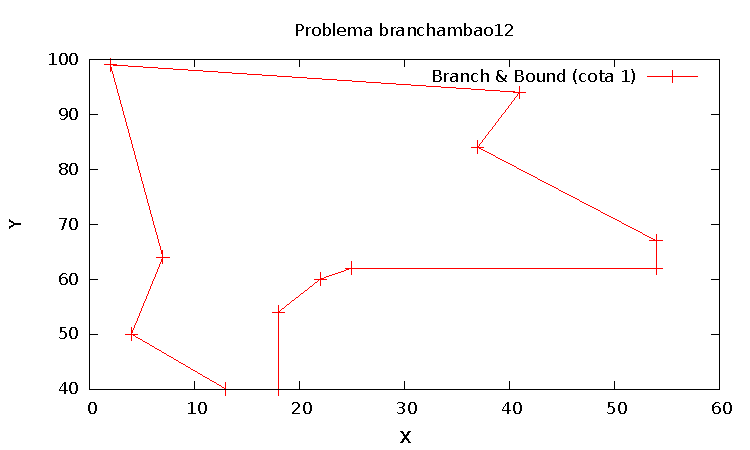
\includegraphics[width=15cm]{img/branchambao12_tsp_1}

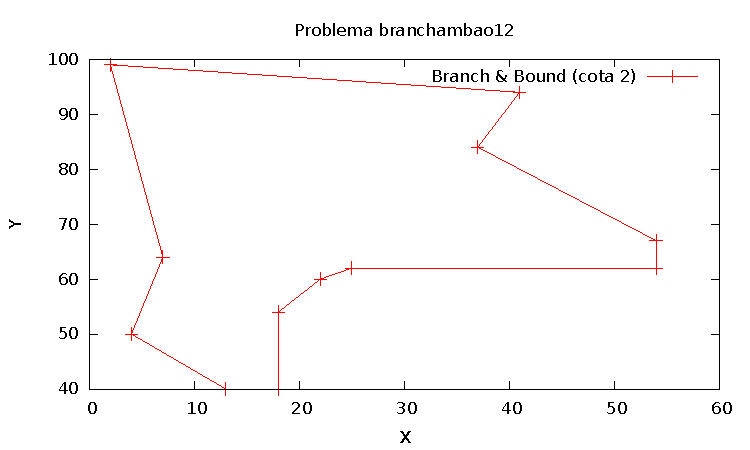
\includegraphics[width=15cm]{img/branchambao12_tsp_2}

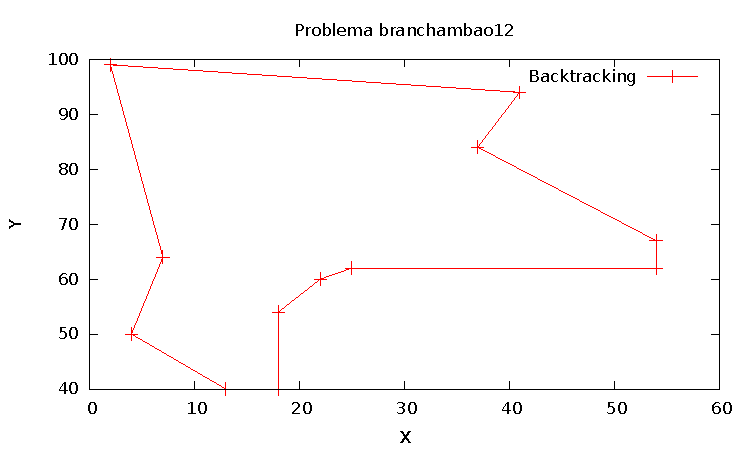
\includegraphics[width=15cm]{img/branchambao12_tsp_3}

En este tercer caso, los tres coinciden. \\

Ahora pasamos a comparar según el tiempo. Debido al elevado tiempo de ejecución de los algoritmos no podemos crear una comparativa con tamaños mucho mayores:

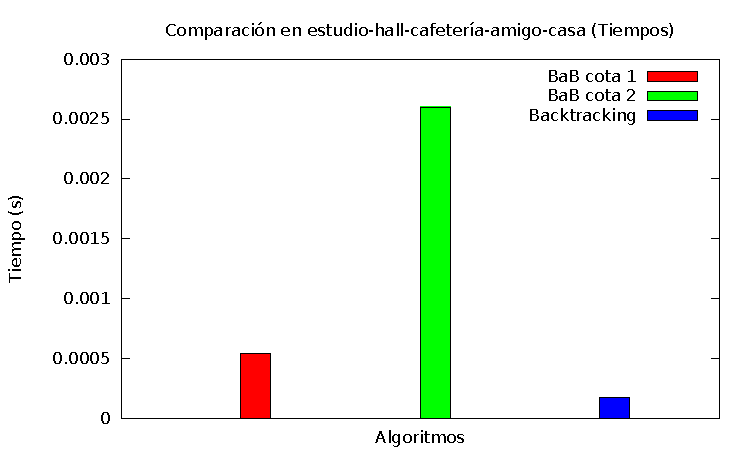
\includegraphics[width=15cm]{img/barras_e-h-c-a-c5_t}

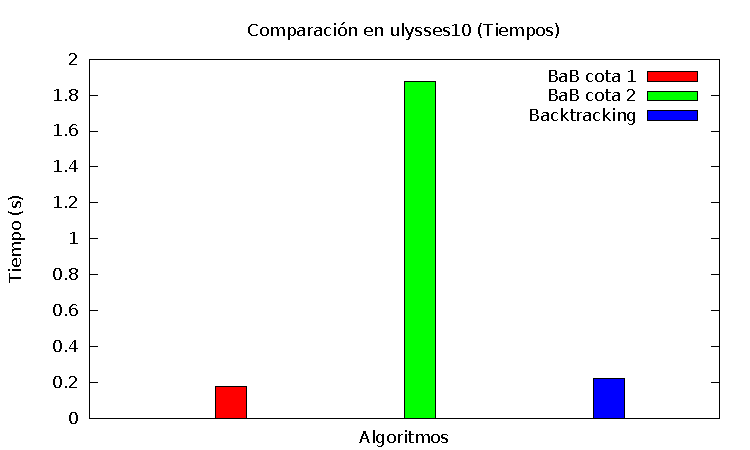
\includegraphics[width=15cm]{img/barras_ulysses10_t}

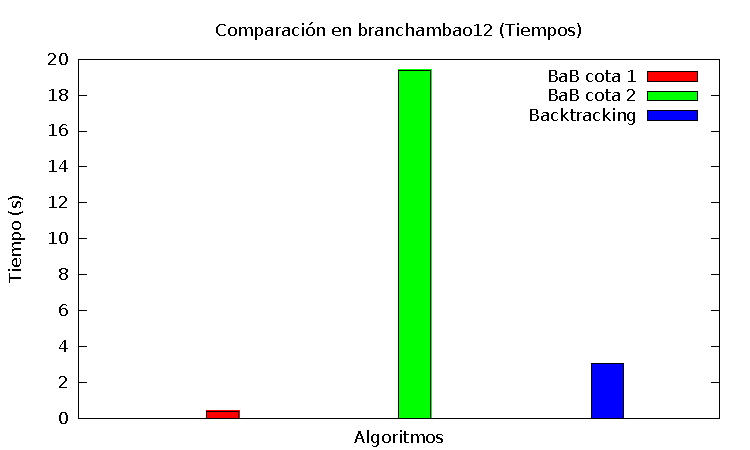
\includegraphics[width=15cm]{img/barras_branchambao12_t}

Con estos mismos ejemplos, comparamos según el número de nodos expandidos:

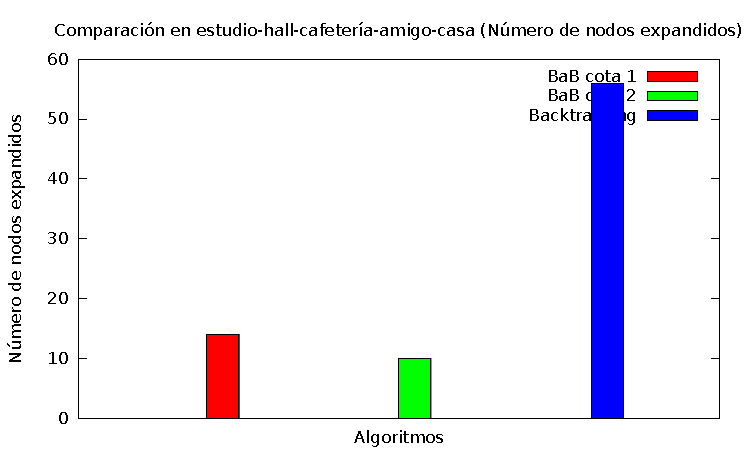
\includegraphics[width=15cm]{img/barras_e-h-c-a-c5_nodos}

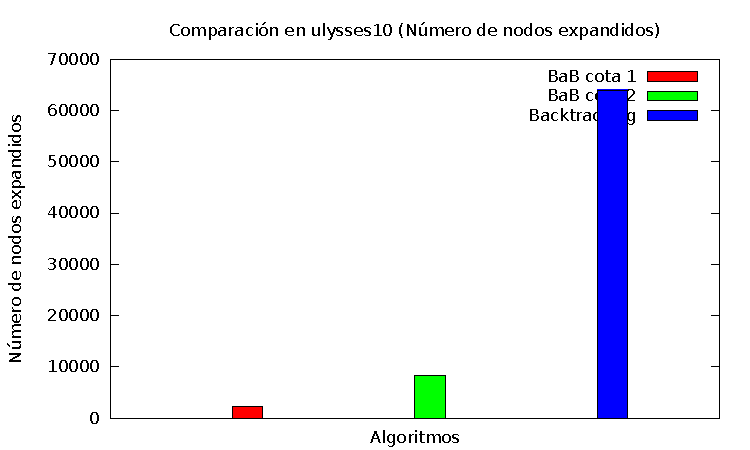
\includegraphics[width=15cm]{img/barras_ulysses10_nodos}

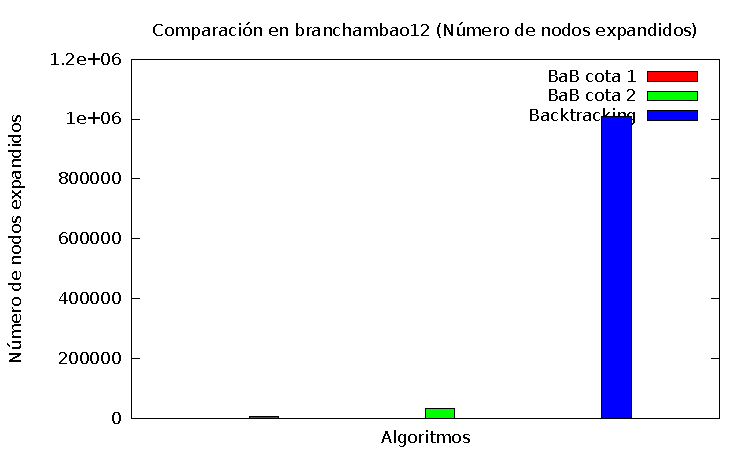
\includegraphics[width=15cm]{img/barras_branchambao12_nodos}

Comparamos según el número de veces que se poda:

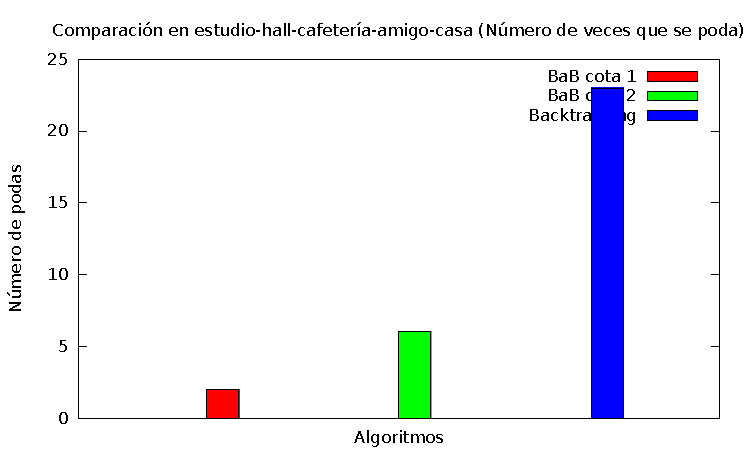
\includegraphics[width=15cm]{img/barras_e-h-c-a-c5_poda}

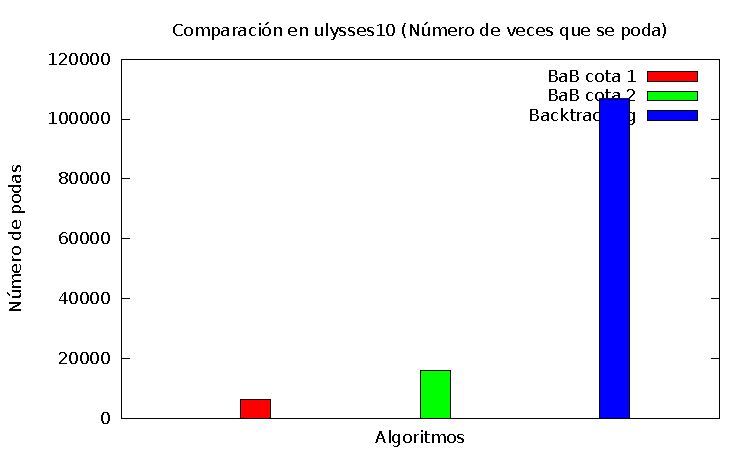
\includegraphics[width=15cm]{img/barras_ulysses10_poda}

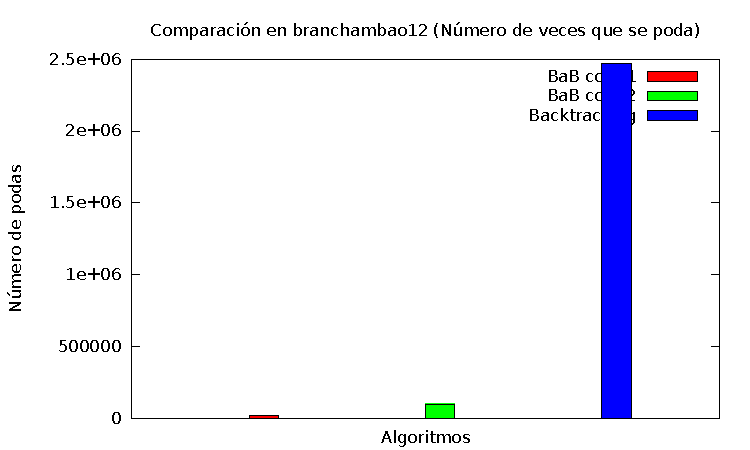
\includegraphics[width=15cm]{img/barras_branchambao12_poda}

Y, solamente para los algoritmos Branch and Bound, observamos el tamaño máximo de nodos vivos en la cola de prioridad:

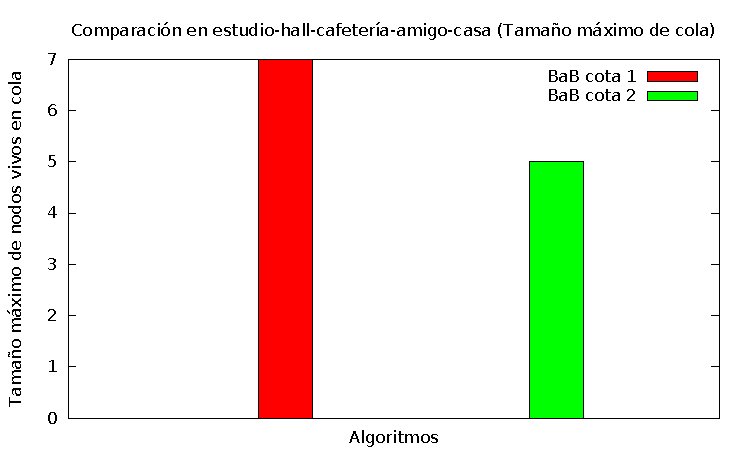
\includegraphics[width=15cm]{img/barras_e-h-c-a-c5_cola}

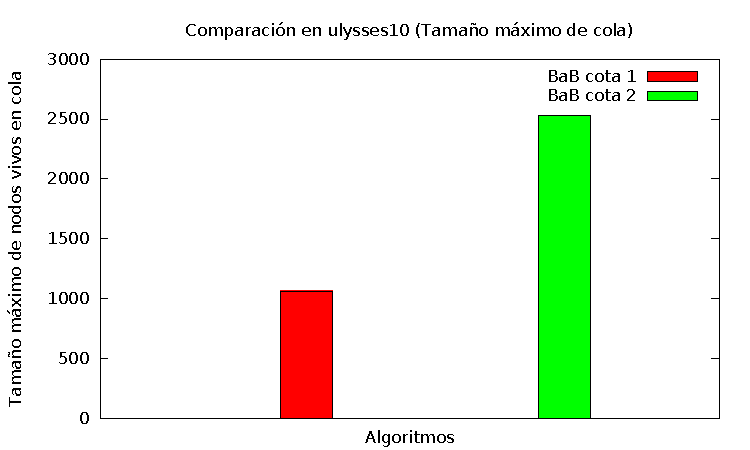
\includegraphics[width=15cm]{img/barras_ulysses10_cola}

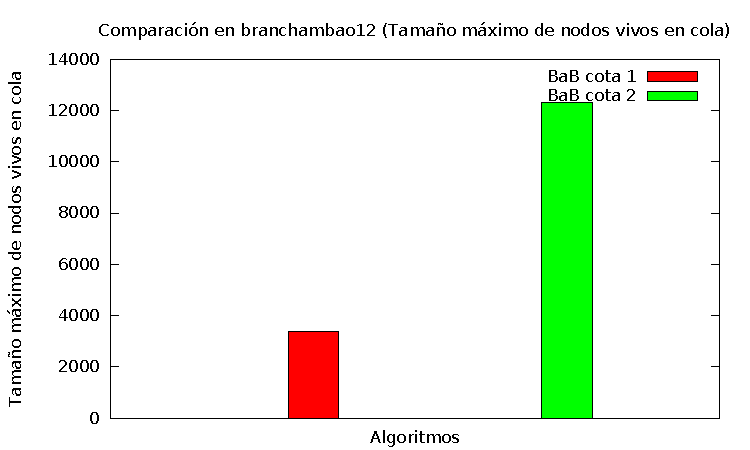
\includegraphics[width=15cm]{img/barras_branchambao12_cola}